\documentclass[12pt,a4paper]{article}

% ── Packages ──────────────────────────────────────────────────────────────────
\usepackage[top=1in, bottom=1in, left=1in, right=1in]{geometry}
\usepackage{graphicx}
\usepackage{amsmath, amssymb}
\usepackage{booktabs}
\usepackage{hyperref}
\usepackage{xcolor}
\usepackage{titlesec}
\usepackage{parskip}
\usepackage{caption}
\usepackage{float}
\usepackage{fancyhdr}
\usepackage{enumitem}
\usepackage{microtype}
\usepackage{array}
\usepackage{tabularx}
\usepackage{mdframed}
\usepackage{colortbl}

% ── Colours ───────────────────────────────────────────────────────────────────
\definecolor{accentblue}{RGB}{30, 80, 160}
\definecolor{lightgray}{RGB}{245, 245, 245}
\definecolor{darkgray}{RGB}{60, 60, 60}
\definecolor{tableheader}{RGB}{30, 80, 160}

% ── Page style ────────────────────────────────────────────────────────────────
\pagestyle{fancy}
\fancyhf{}
\rhead{\textcolor{accentblue}{\small Denoising Autoencoder -- Assignment 3}}
\lhead{\textcolor{darkgray}{\small Question 2.1}}
\cfoot{\thepage}
\renewcommand{\headrulewidth}{0.4pt}

% ── Section formatting ────────────────────────────────────────────────────────
\titleformat{\section}
  {\large\bfseries\color{accentblue}}
  {}
  {0em}
  {}[\color{accentblue}\titlerule]

\titleformat{\subsection}
  {\normalsize\bfseries\color{darkgray}}
  {}
  {0em}
  {}

\titlespacing{\section}{0pt}{12pt}{6pt}
\titlespacing{\subsection}{0pt}{8pt}{4pt}

% ── Hyperref ──────────────────────────────────────────────────────────────────
\hypersetup{
  colorlinks=true,
  linkcolor=accentblue,
  urlcolor=accentblue
}

% ─────────────────────────────────────────────────────────────────────────────
\begin{document}

% ==================== PAGE 2: ARCHITECTURE ===================================
\newpage
\section{Model Architecture}

The model is a symmetric convolutional autoencoder implemented in PyTorch. It
consists of two sub-networks: an \textbf{Encoder} that compresses the input
image into a compact latent representation, and a \textbf{Decoder} that
reconstructs the clean image from that representation. Both experiments share
\emph{identical} architecture; only the training inputs differ.

\subsection{Encoder}

The encoder maps a $3 \times 64 \times 64$ RGB image to a bottleneck tensor
of shape $256 \times 8 \times 8$ through three successive
\textit{Conv2d $\to$ BatchNorm $\to$ LeakyReLU $\to$ MaxPool2d} blocks,
each doubling the channel depth while halving the spatial resolution.

\vspace{4pt}
\renewcommand{\arraystretch}{1.35}
\begin{center}
\begin{tabular}{clcccc}
\toprule
\textbf{Block} & \textbf{Operation} & \textbf{In Ch.} & \textbf{Out Ch.}
               & \textbf{Kernel/Stride} & \textbf{Output Shape} \\
\midrule
1 & Conv2d + BN + LeakyReLU(0.1) & 3   & 64  & $3\times3$, pad=1 & $64\times64\times64$ \\
  & MaxPool2d                    & --  & --  & $2\times2$        & $64\times32\times32$ \\
\midrule
2 & Conv2d + BN + LeakyReLU(0.1) & 64  & 128 & $3\times3$, pad=1 & $128\times32\times32$ \\
  & MaxPool2d                    & --  & --  & $2\times2$        & $128\times16\times16$ \\
\midrule
3 & Conv2d + BN + LeakyReLU(0.1) & 128 & 256 & $3\times3$, pad=1 & $256\times16\times16$ \\
  & MaxPool2d                    & --  & --  & $2\times2$        & $256\times8\times8$ \\
\bottomrule
\end{tabular}
\end{center}

\textbf{LeakyReLU(0.1):} Standard ReLU permanently kills neurons with negative
pre-activations. A small negative slope of 0.1 allows gradients to flow for
negative inputs, preventing dead neurons and producing richer latent encodings.

\textbf{BatchNorm2d:} Applied after each convolution to normalise feature maps
per channel. This accelerates convergence, reduces internal covariate shift,
and provides mild regularisation -- valuable when training on limited data.

\subsection{Decoder}

The decoder inverts the spatial compression using three \texttt{ConvTranspose2d}
(learnable upsampling) blocks, each immediately followed by an additional
\texttt{Conv2d} refinement layer.

\vspace{4pt}
\begin{center}
\begin{tabular}{clcccc}
\toprule
\textbf{Block} & \textbf{Operation} & \textbf{In Ch.} & \textbf{Out Ch.}
               & \textbf{Kernel/Stride} & \textbf{Output Shape} \\
\midrule
1 & ConvTranspose2d + BN + LeakyReLU & 256 & 128 & $2\times2$, stride=2 & $128\times16\times16$ \\
  & Conv2d + LeakyReLU (refine)       & 128 & 128 & $3\times3$, pad=1    & $128\times16\times16$ \\
\midrule
2 & ConvTranspose2d + BN + LeakyReLU & 128 & 64  & $2\times2$, stride=2 & $64\times32\times32$ \\
  & Conv2d + LeakyReLU (refine)       & 64  & 64  & $3\times3$, pad=1    & $64\times32\times32$ \\
\midrule
3 & ConvTranspose2d + BN + LeakyReLU & 64  & 32  & $2\times2$, stride=2 & $32\times64\times64$ \\
  & Conv2d + Sigmoid (output)         & 32  & 3   & $3\times3$, pad=1    & $3\times64\times64$ \\
\bottomrule
\end{tabular}
\end{center}

\subsection{Why Convolutional Refinement Layers After Each Upsampling Step?}

A common simplification is to use only \texttt{ConvTranspose2d} with no
follow-up convolution. While this reduces parameter count, it introduces a
well-documented problem -- \textbf{checkerboard artefacts}: because
\texttt{ConvTranspose2d} with stride 2 distributes values unevenly across the
output grid (whenever kernel size is not a perfect multiple of the stride),
the result shows a characteristic grid-like pattern that persists throughout
training.

The additional $3\times3$ \texttt{Conv2d} inserted \emph{after} each
\texttt{ConvTranspose2d} serves three purposes:

\begin{enumerate}[leftmargin=*, itemsep=3pt]
  \item \textbf{Artefact suppression:} The convolution re-mixes neighbouring
        pixels, smoothing the uneven checkerboard pattern before the signal
        is passed to the next resolution scale.
  \item \textbf{Feature refinement:} Extra learnable parameters at each
        spatial scale allow the decoder to reconstruct finer textures and
        structural detail rather than only coarse outlines.
  \item \textbf{Additional non-linearity:} Paired with LeakyReLU, each
        refinement layer increases the decoder's expressive capacity without
        any additional spatial cost.
\end{enumerate}

The final layer uses \textbf{Sigmoid} to constrain all output pixel values to
$[0,1]$, matching the normalised range produced by
\texttt{transforms.ToTensor()}.


% ==================== PAGE 3: EXPERIMENTS ====================================
\newpage
\section{Experiments and Results}

\subsection{Experiment 1 -- Standard Reconstruction Autoencoder}

In the first experiment, the autoencoder was trained to reconstruct its
\emph{clean} input directly: the same image served as both the network input
and the reconstruction target.

\begin{mdframed}[backgroundcolor=lightgray, linecolor=accentblue, linewidth=0.8pt,
                 innerleftmargin=10pt, innerrightmargin=10pt,
                 innertopmargin=6pt, innerbottommargin=6pt]
\textbf{Training objective:}
\[
  \mathcal{L}_{\text{MSE}} = \frac{1}{N}\sum_{i=1}^{N}
    \bigl\| f_\theta(x_i) - x_i \bigr\|^2
\]
Optimiser: Adam, $lr=10^{-2}$, 50 epochs, batch size 32.
\end{mdframed}

\vspace{6pt}
This experiment establishes the \emph{upper-bound} reconstruction quality: a
model that receives clean images and is only asked to reproduce them.
After 50 epochs on Tiny-ImageNet-10, the model achieved a test-set SSIM of
\textbf{71\%}, confirming that the architecture has sufficient capacity to
learn compact and recoverable image representations.

\subsection{Experiment 2 -- Denoising Autoencoder (DAE)}

In the second experiment, the autoencoder was re-trained as a proper denoising
model. Gaussian noise was injected into each image before it was passed to the
encoder, while the \emph{clean} original image remained the reconstruction
target.

\vspace{6pt}
The DAE achieved a test-set SSIM of \textbf{70\%} -- only 1 percentage point
below the standard autoencoder, despite the significantly harder task of
recovering clean images from corrupted inputs. This demonstrates that the
architecture generalises well to the denoising objective and that the MSE
loss correctly guides the network to suppress noise while preserving
structural content.

\subsection{Reconstruction Trio Visualisation}

Figure~\ref{fig:trio} shows a representative sample from the test set,
illustrating the full pipeline: the original clean image, the
noise-corrupted input, and the model's denoised output.

\begin{figure}[H]
  \centering
  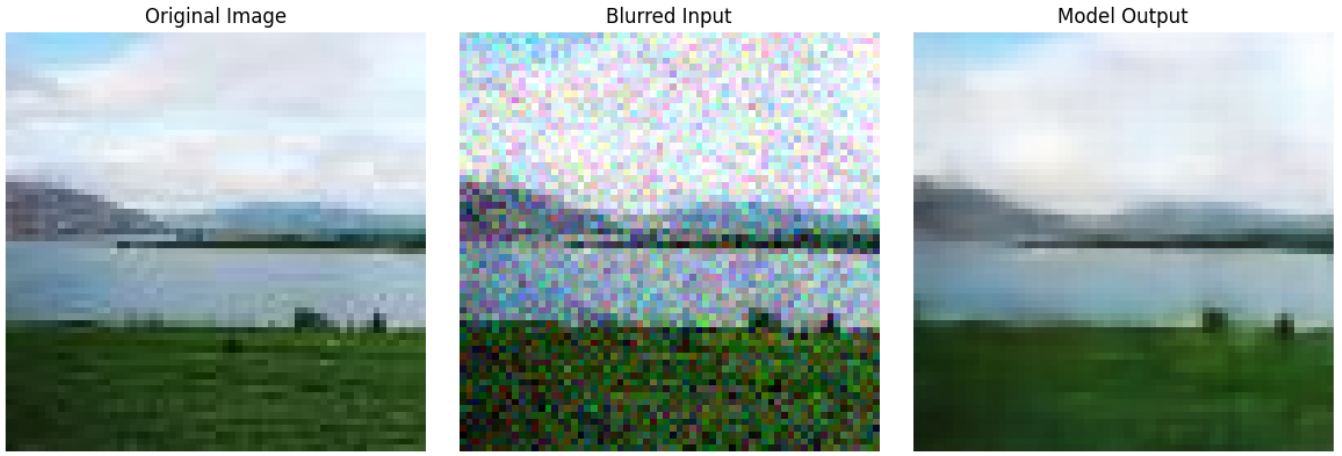
\includegraphics[width=0.96\textwidth]{autoencoder_result.png}
  \caption{%
    \textbf{Reconstruction Trio.}
    \textit{Left:} Original clean image from Tiny-ImageNet-10.
    \textit{Centre:} Noisy input after Gaussian noise corruption
    ($\mu = 0,\, \sigma = 0.1$).
    \textit{Right:} Denoised output produced by the trained DAE.
    The model successfully recovers large-scale structure (sky, mountains,
    water, grass) and suppresses pixel-level noise, achieving an average
    SSIM of 70\% across the full test set.
  }
  \label{fig:trio}
\end{figure}


% ==================== PAGE 4: METRIC DISCUSSION ==============================
\newpage
\section{Loss Function and Evaluation Metric}

\subsection{Why MSE is the Right Loss for Image Reconstruction}

Mean Squared Error is the canonical training loss for autoencoders, and its
choice here is well-motivated on both practical and statistical grounds.

\begin{enumerate}[leftmargin=*, itemsep=5pt]

  \item \textbf{Pixel-wise intensity agreement.}
        MSE penalises every pixel independently. When the target is a clean
        image and the prediction is corrupted or blurred, large per-pixel
        deviations receive large squared penalties, directly incentivising the
        network to produce sharp, accurate reconstructions.

  \item \textbf{Smooth, well-conditioned gradients.}
        The squared error is differentiable everywhere and its gradient,
        \[
          \nabla_{\hat{x}}\,\mathcal{L}_\text{MSE}
            = \frac{2}{N}(\hat{x} - x),
        \]
        scales linearly with prediction error. This makes optimisation with
        Adam stable and avoids the gradient pathologies that arise when using
        cross-entropy on continuous pixel values.

  \item \textbf{Statistical consistency with Gaussian noise.}
        Adding $\varepsilon \sim \mathcal{N}(0, \sigma^2)$ to images means
        the maximum-likelihood estimator for the clean signal is \emph{exactly}
        the MSE minimiser. The loss is therefore statistically consistent with
        the noise model used in this experiment -- a property not shared by,
        e.g., binary cross-entropy.

  \item \textbf{Simplicity and interpretability.}
        Unlike perceptual losses or adversarial objectives, MSE requires no
        additional networks, has no hyperparameters to tune, and its value
        has a direct intuitive meaning: the average squared pixel distance
        between prediction and target.

\end{enumerate}

\subsection{Why SSIM is a Better Evaluation Metric Than $R^2$}

\textbf{What SSIM measures.}
The Structural Similarity Index Measure compares two image patches along three
perceptually meaningful axes -- luminance, contrast, and structure:
where $\mu$, $\sigma$, and $\sigma_{x\hat{x}}$ are the local mean,
standard deviation, and cross-covariance respectively.
A score of 1.0 indicates perfect identity; 0.0 indicates no perceptual
similarity.

\medskip
\noindent\textbf{Limitations of $R^2$ for image quality assessment.}

While suitable for tabular regression tasks, it is a poor image quality metric
for three reasons:

\begin{enumerate}[leftmargin=*, itemsep=5pt]
  \item \textbf{Global, not structural.}
        $R^2$ aggregates error uniformly over all pixels. A reconstruction
        that is slightly wrong everywhere receives the same score as one that
        is perfect in most regions but severely wrong in a small area -- yet
        a human observer would judge these cases very differently.

  \item \textbf{Insensitive to perceptual quality.}
        A mildly brightness-shifted copy of the original can yield a low $R^2$
        yet look nearly identical to the original. Conversely, a blurry
        average-coloured image may score high while appearing perceptually
        degraded. $R^2$ does not account for edges, textures, or local
        contrast, which are the primary cues human vision uses.

  \item \textbf{Uninformative negative values.}
        For image reconstruction, $R^2$ can easily turn negative when the
        model underperforms a trivial mean predictor. This provides no
        actionable insight about \emph{which} visual properties failed
        and makes cross-experiment comparison unreliable.
\end{enumerate}

\noindent SSIM is explicitly designed for images. It is sensitive to edge
alignment, texture fidelity, and local contrast -- the exact properties that
determine perceived reconstruction quality. Its bounded range (practically
$[0, 1]$ for natural images) makes scores directly comparable across
experiments, architectures, and noise levels.

\section*{Conclusion}

Two experiments were conducted on Tiny-ImageNet-10 using a convolutional
autoencoder with a Conv--BN--LeakyReLU--MaxPool encoder and a
ConvTranspose--Conv(refine) decoder. The standard reconstruction autoencoder
achieved an SSIM of \textbf{71\%}; the denoising variant, trained on
Gaussian-corrupted inputs ($\sigma=0.1$), achieved \textbf{70\%} -- demonstrating
effective noise suppression with negligible loss in reconstruction quality.
The choice of MSE as the training loss is statistically motivated by the
Gaussian noise model, and SSIM provides the perceptually meaningful evaluation
that $R^2$ cannot replicate for image data.

\end{document}
